\documentclass[12pt,a4paper]{article}
\usepackage{ctex}
\usepackage{amsmath,amscd,amsbsy,amssymb,latexsym,url,bm,amsthm}
\usepackage{epsfig,graphicx,subfigure}
\usepackage{enumitem,balance}
\usepackage{wrapfig}
\usepackage{mathrsfs,euscript}
\usepackage[usenames]{xcolor}
\usepackage{hyperref}
\usepackage[vlined,ruled,linesnumbered]{algorithm2e}
\usepackage{array}
\hypersetup{colorlinks=true,linkcolor=black}

\newtheorem{theorem}{Theorem}
\newtheorem{lemma}[theorem]{Lemma}
\newtheorem{proposition}[theorem]{Proposition}
\newtheorem{corollary}[theorem]{Corollary}
\newtheorem{exercise}{Exercise}
\newtheorem*{solution}{Solution}
\newtheorem{definition}{Definition}
\theoremstyle{definition}

\renewcommand{\thefootnote}{\fnsymbol{footnote}}

\newcommand{\postscript}[2]
 {\setlength{\epsfxsize}{#2\hsize}
  \centerline{\epsfbox{#1}}}

\renewcommand{\baselinestretch}{1.0}

\setlength{\oddsidemargin}{-0.365in}
\setlength{\evensidemargin}{-0.365in}
\setlength{\topmargin}{-0.3in}
\setlength{\headheight}{0in}
\setlength{\headsep}{0in}
\setlength{\textheight}{10.1in}
\setlength{\textwidth}{7in}
\makeatletter \renewenvironment{proof}[1][Proof] {\par\pushQED{\qed}\normalfont\topsep6\p@\@plus6\p@\relax\trivlist\item[\hskip\labelsep\bfseries#1\@addpunct{.}]\ignorespaces}{\popQED\endtrivlist\@endpefalse} \makeatother
\makeatletter
\renewenvironment{solution}[1][Solution] {\par\pushQED{\qed}\normalfont\topsep6\p@\@plus6\p@\relax\trivlist\item[\hskip\labelsep\bfseries#1\@addpunct{.}]\ignorespaces}{\popQED\endtrivlist\@endpefalse} \makeatother

\begin{document}
\noindent

%========================================================================
\noindent\framebox[\linewidth]{\shortstack[c]{
\Large{\textbf{Lab07-Amortized Analysis}}\vspace{1mm}\\
CS214-Algorithm and Complexity, Xiaofeng Gao, Spring 2020.}}
\begin{center}
\footnotesize{\color{red}$*$ If there is any problem, please contact TA Shuodian Yu. }

\footnotesize{\color{blue}$*$ Name:Hanzhang Yang  \quad Student ID:518030910022 \quad Email: linqinluli@sjtu.edu.cn}
\end{center}
\begin{enumerate}
	\item For the TABLE-DELETE Operation in Dynamic Tables, suppose we construct a table by multiplying its size by $\frac 23$ when the load factor drops below $\frac 13$. Using \emph{Potential Method} to prove that the amortized cost of a TABLE-DELETE that uses this strategy is bounded above by a constant.
	
	\textbf{Solution.}
	
		$$\Phi(T)=size[T]-num[T]$$

	\textbf{case 1: no contraction}

	The amortized cost is:

	\begin{align*}  
		\hat{C_i} &= C_i+\Phi_i-\Phi_{i-1} \\  
	   &= 1+(size_i-num_i)-(size_{i-1}-num_{i-1})  \\  
	   &=2   
	  \end{align*} 

	\textbf{case 2: a contraction was triggered}

	The amortized cost is:

	\begin{align*}  
		\hat{C_i} &= C_i+\Phi_i-\Phi_{i-1} \\  
	   &= num_{i-1}+(size_i-num_i)-(size_{i-1}-num_{i-1})  \\  
	   &=num_{i-1}+(\frac{2}{3}size_{i-1}-num_{i-1}+1)-(size_{i-1}-num_{i-1})\\
	&=num_{i-1}-\frac{1}{3}size_{i-1}+1\leftarrow\quad num_{i-1}=\frac{1}{3}size_{i-1}\\
	&=1
	\end{align*} 

	Therefore the cost of a TABLE-DELETE is bounded above by a constant.

	\item A \textbf{multistack} consists of an infinite series of stacks $S_0, S_1, S_2,\cdots$, where the $i^{th}$ stack $S_i$ can hold up to $3^i$ elements. Whenever a user attempts to push an element onto any full stack $S_i$, we first pop all the elements off $S_i$ and push them onto stack $S_{i+1}$ to make room. (Thus, if $S_{i+1}$ is already full, we first recursively move all its members to $S_{i+2}$ .) An illustrative example is shown in Figure \ref{Fig-MultiStack}. Moving a single element from one stack to the next takes $O(1)$ time. If we push a new element, \underline{we always intend to push it in stack $S_0$}.

	\begin{figure}[!htbp]
	\centering
	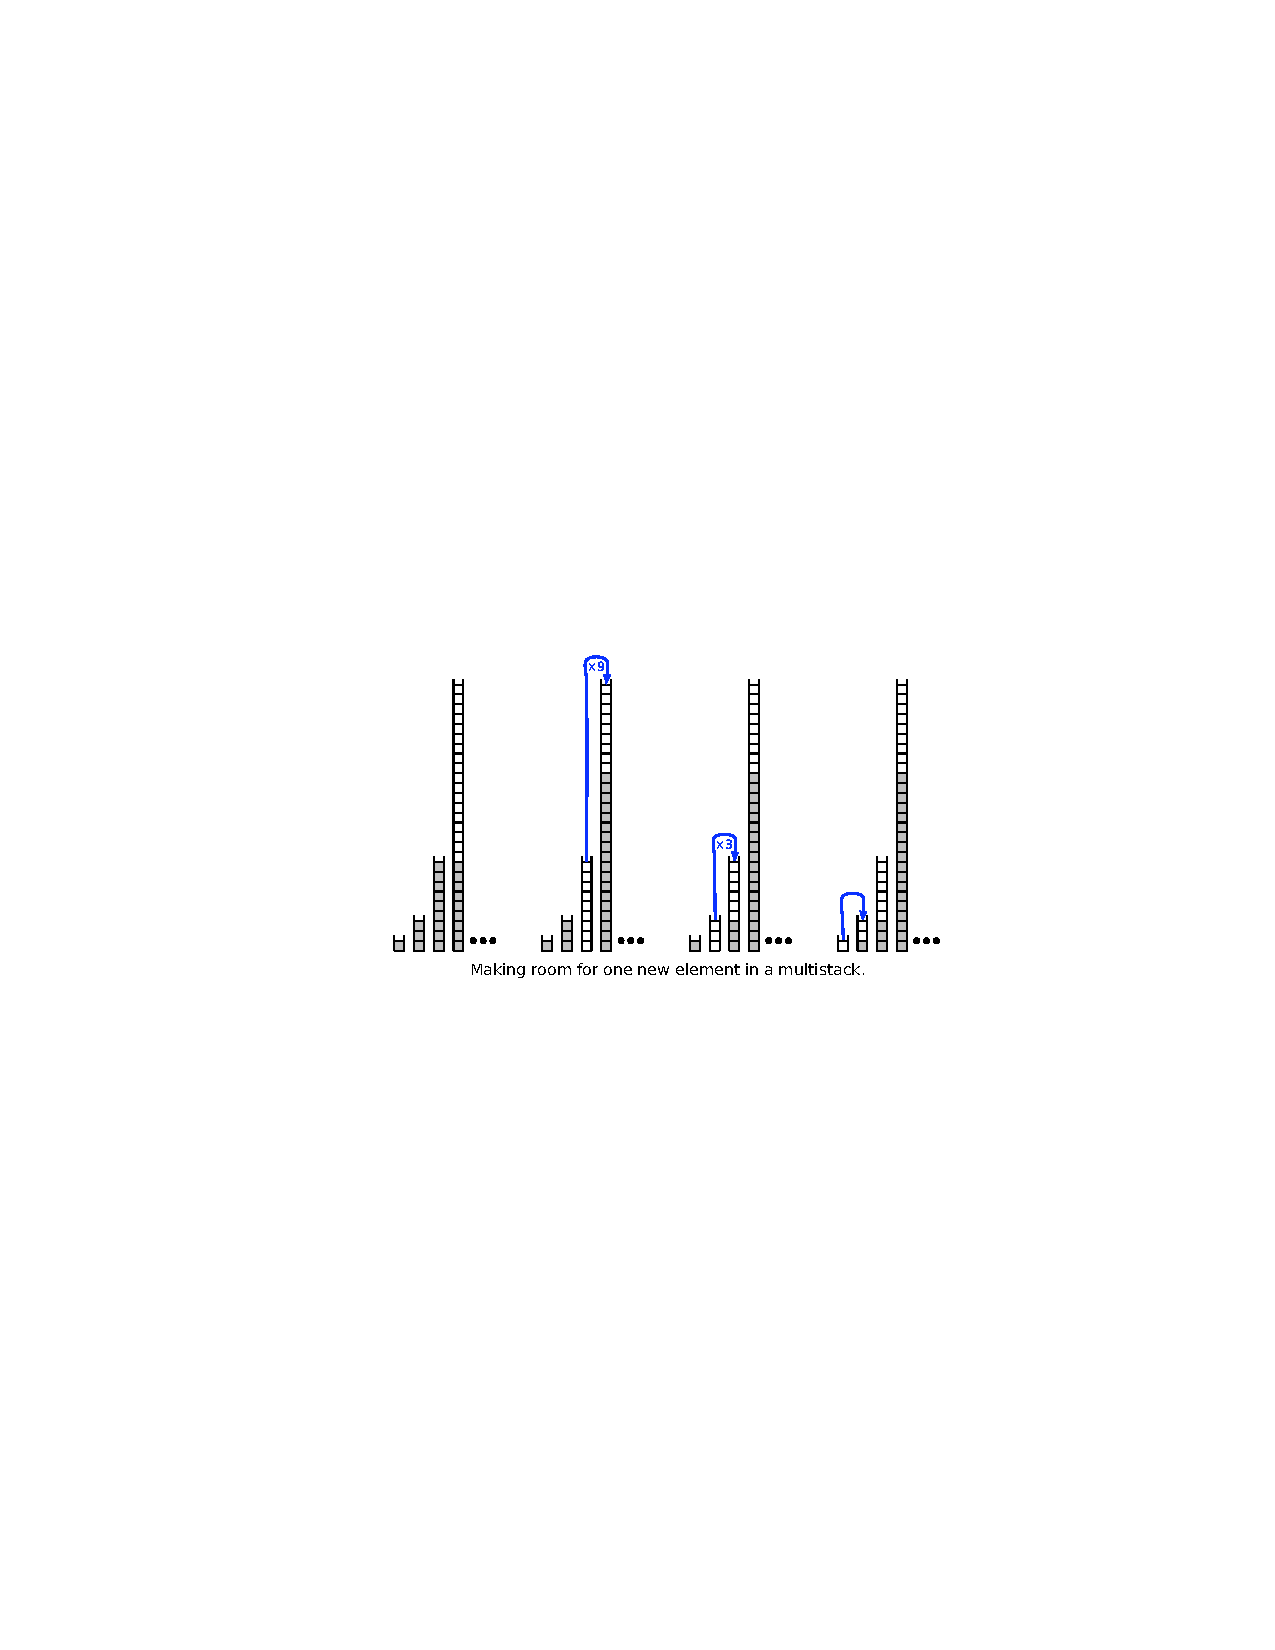
\includegraphics[width=0.5\textwidth]{Fig-MultiStack.pdf}
	\caption{An example of making room for one new element in a multistack.}
	\label{Fig-MultiStack}
	\end{figure}

	\newpage

	$$\sum_{i=0}{i=k}$$
    \begin{enumerate}
        \item In the worst case, how long does it take to push a new element onto a multistack containing $n$ elements?
        \item Prove that the amortized cost of a push operation is $O(\log n)$ by \emph{Aggregation Analysis}.
        \item {\color{red}(Optional Subquestion with Bonus)} Prove that the amortized cost of a push operation is $O(\log n)$ by \emph{Potential Method}.
    \end{enumerate}
	
	
	\textbf{Solution.}

	(a) The worst case is when we push a new element, the $n$ elements in the multistack are filled with the first $k$ stacks.
		And all elements are needed to be moved. The time cost is $O(n)$.

	(b) The worst time $T(n)$ in total for a sequence of $n$ operations is when the $n$ elements are stoed in the $i_{th}$ stack.

	All the elemens pushed from $stack_1$ to $stack_i$ and cost $O(i)$ time.

	And it's clear that $n=\frac{3^{i-1}-1}{2}$. Thus $i=O(\log n)$.

	Thus the amortized cost of a push operation is $\frac{nO(\log n)}{n}=O(\log n)$
	\item Given a graph $G = (V, E)$, and let $V'$ be a strict subset of $V$. Prove the following propositions.
	
	\begin{enumerate}
		\item Let $T$ be a minimum spanning tree of a $G$. Let $T'$ be the subgraph of $T$ induced by $V'$, and let $G'$ be the subgraph of $G$ induced by $V'$. Then $T'$ is a minimum spanning tree of $G'$ if $T'$ is connected.
		\item Let $e$ be a minimum weight edge which connects $V'$ and $V \setminus V'$. There exists a minimum weight spanning tree which contains e.
	\end{enumerate}
\end{enumerate}

\textbf{Solution.}

(a) Assume $T'$ is not a minimum spanning tree of $G'$ if $T'$ is connected.

And there must exist an edge $e_2\in G'$ that own smaller weight than the edge $e_1\in T'$. 

For $T$, the reason why $e_2\notin T$ is that $e_2$ forms a circle if we add $e_2$ in $T$. Thus in the connected tree $T'$, the edge $e_2$ must form a circle in $T'$.

Therefore $T'$ is a minimum spanning tree of $G'$ if $T'$ is connected.

(b) Assume all the minimum spanning tree in $G$ don't contain the minimum weight edge $(u,v)$.

Let $T$ one of the minimum spanning tree in $G$. If we joing $(u,v)$ to $T$, there must exist a circle containing $(u, v)$. And for $T$ is a spanning tree, there must exist another edge $(u', v')$ that $u'\in V'$ and $v'\in V/V'$. Thus $u$ is connected with $u'$
and $v$ is connected with $v'$.

Deleting $(u', v')$ will eliminate the circle. And add $(u, v)$ to $T$ will form another spanning tree whose weight is smaller than that containing $(u', v')$.

Therefore there exists a minimum weight spanning tree which contains $e$.

\vspace{2.1cm}
\textbf{Remark:} Please include your .pdf, .tex files for uploading with standard file names.


%========================================================================
\end{document}
